%Use one of the two documentclass lines depending on aspect ratio needed
% for 4x3 aspect ratio slides
%\documentclass{beamer}
%for 16x9 (modern wide screen) aspect ratio slides
\documentclass[aspectratio=169]{beamer}

% Oxford Maths theming
\usetheme{oxfordmaths}

% Set author etc info
\title[Automated Parallel Goal-Based Adaptivity] %short version of title for slide footer
{Automated Parallel Goal-Based Adaptivity} %full title for titlepage
\author{Yue Wu \\ Supervisor: Prof.\ Patrick Farrell}
\institute{Mathematical Institute\\University of Oxford}
\date[5 June 2026]  %short date for slide footer
{MSc Dissertation Presentation, June 2026} %main date for title page,
                        %can overload it to show say 'Conference X, Date Y'

% Macros
\newcommand{\R}{\mathbb{R}}
\newcommand{\Vh}{V_h}
\newcommand{\Vhe}{V_h^{(2)}}
\newcommand{\inner}[2]{\langle #1, #2 \rangle}

\begin{document}


% --- Title ---
\begin{frame}[plain]
    \titlepage
\end{frame}


% --- Outline ---
\begin{frame}{Outline}
    \tableofcontents[hideallsubsections]
\end{frame}


% --- Motivation ---
\section{Motivation}
\begin{frame}{Motivation: Error Analysis}
\vspace{0.2em}
    \centering
    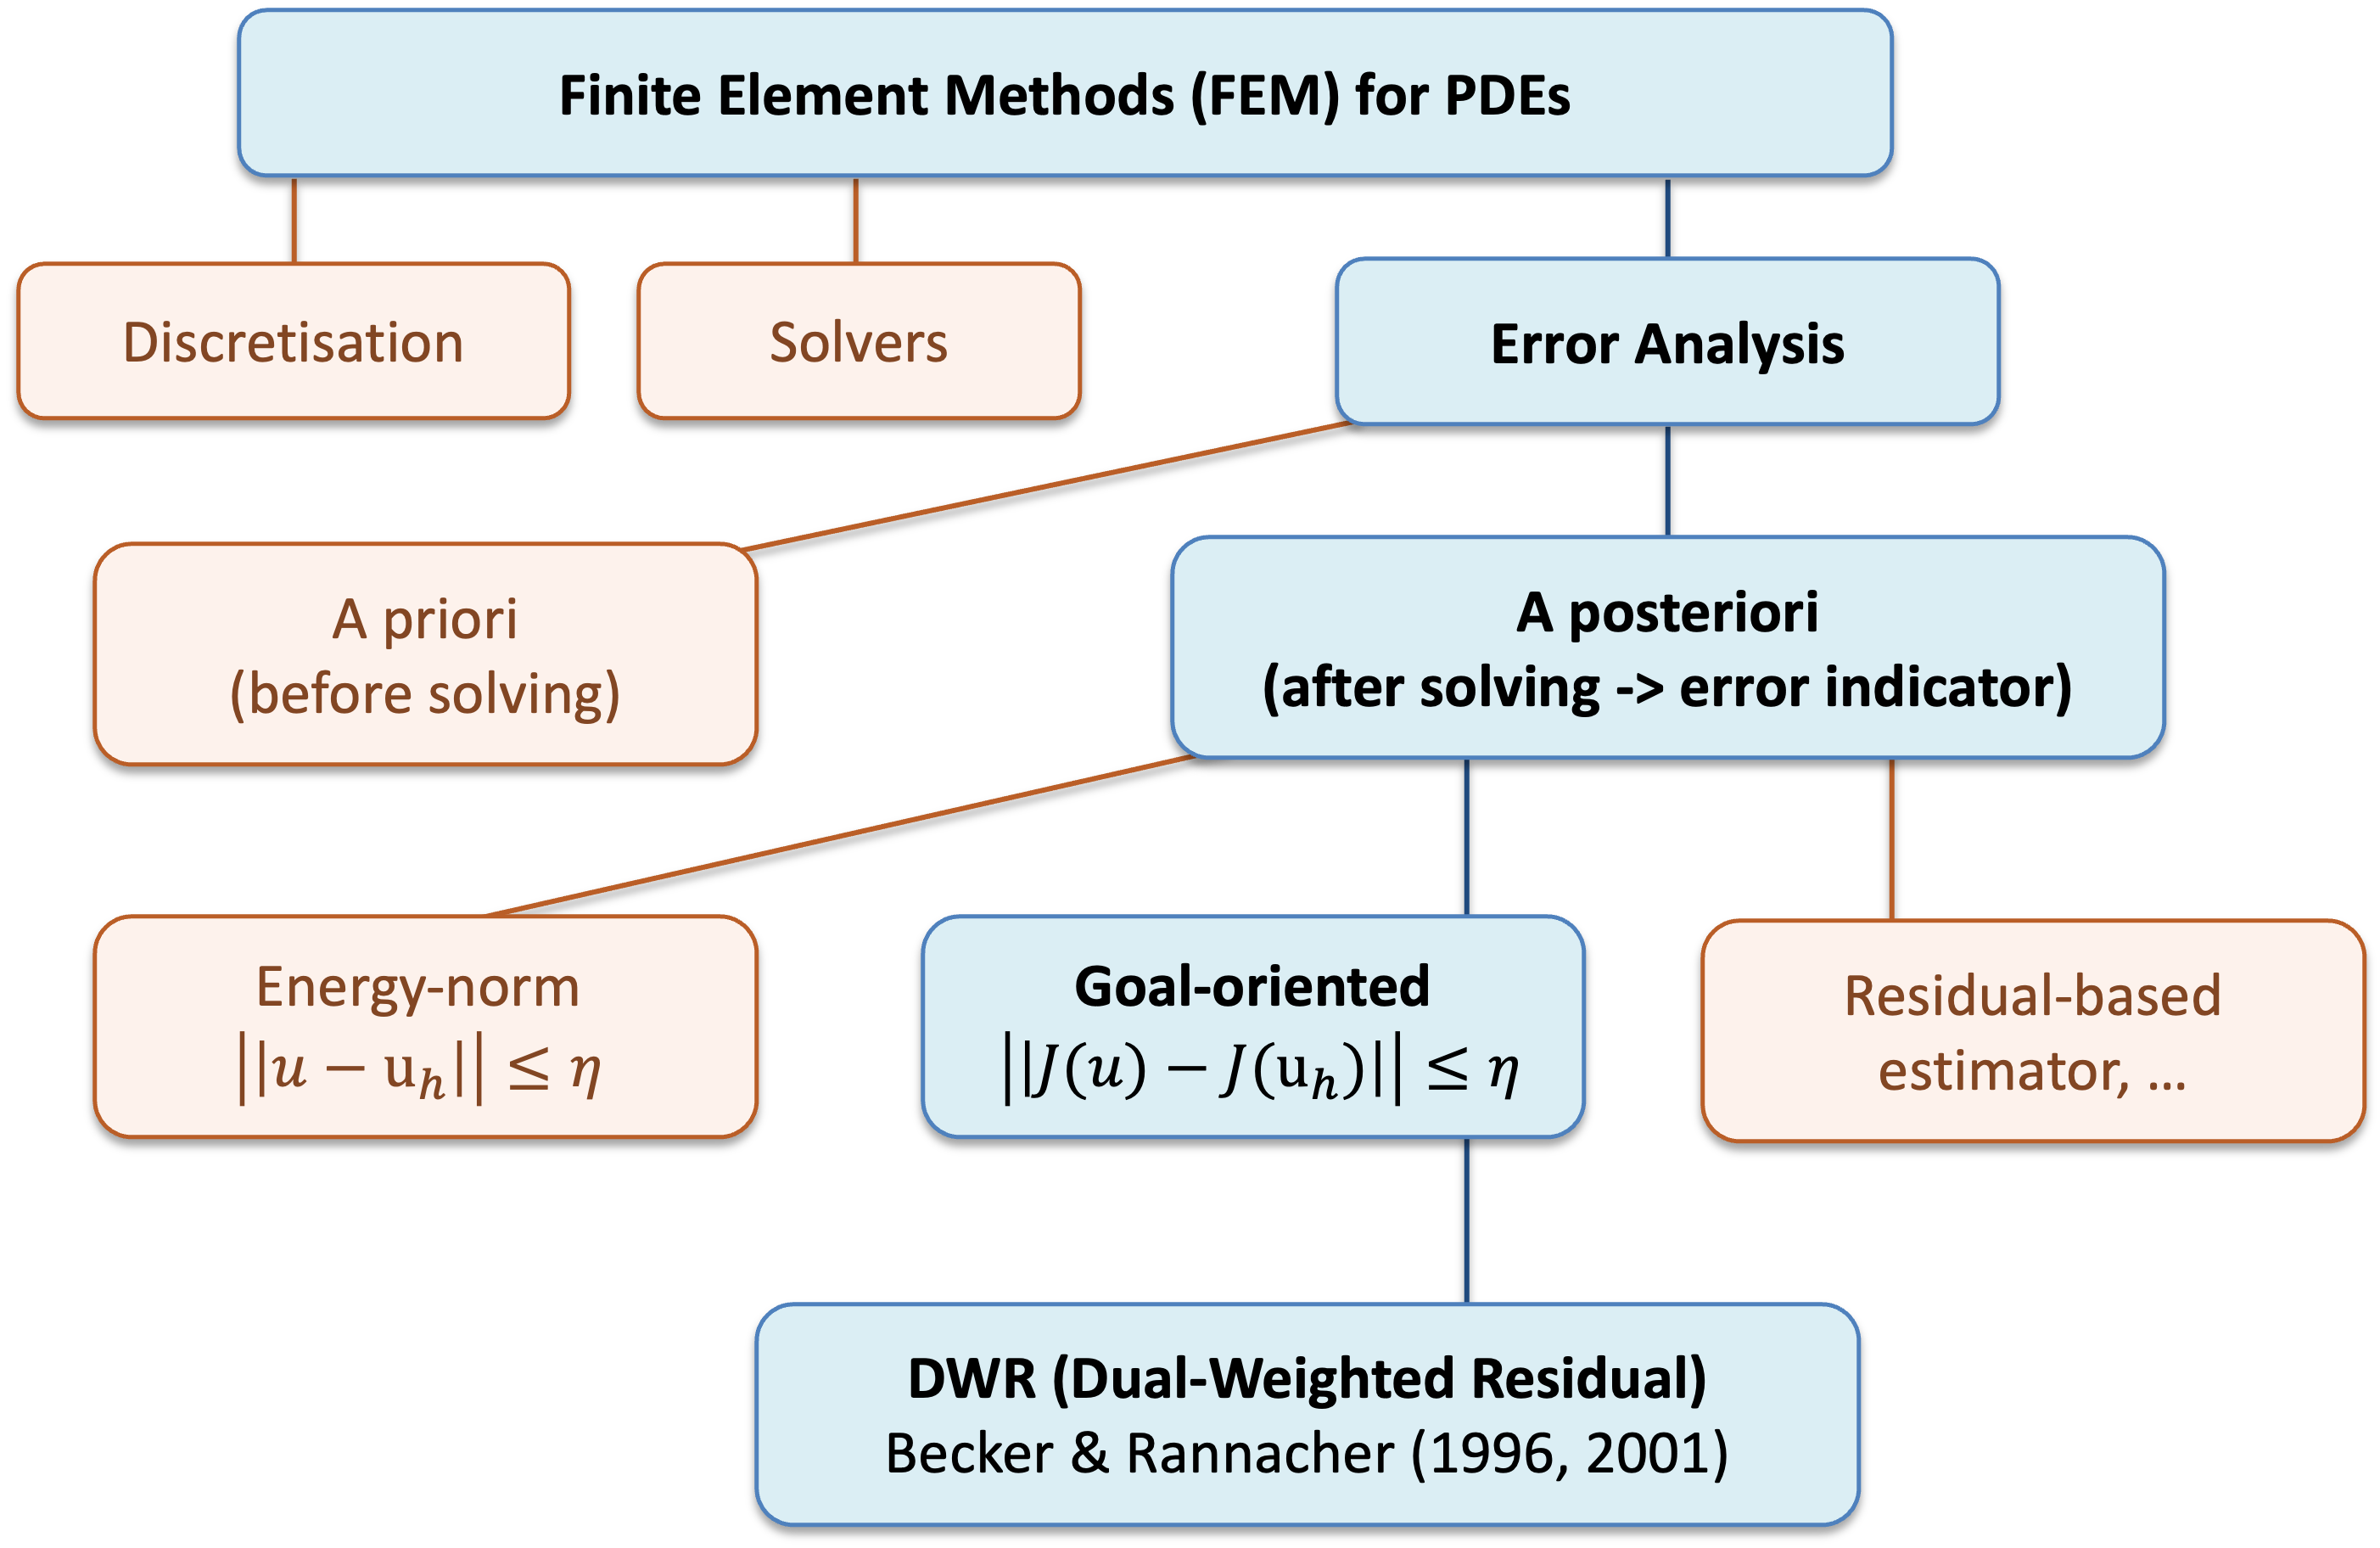
\includegraphics[width=0.75\linewidth]{framework.png}

    % \vspace{0.4em}
    % \begin{block}{Simple example}
    % For the heat equation, \(J(u)\) may be the temperature averaged over a sensor region at final time.
    % \end{block}
\end{frame}



% --- Problem Formulation ---
\section{Dual-Weighted Residual Method}
\begin{frame}{DWR: Problem Formulation}
    \begin{itemize}
        \item \textbf{Primal problem:} Find the exact solution $u \in V$ such that 
        \vspace{-0.5em}
        $$F(u; v) = 0 \quad \forall v \in V.$$
        
        \item \textbf{Finite Element discretisation:} Find the discrete approximation $u_h \in V_h$ s.t.
        \vspace{-0.5em}
        $$F(u_h; v_h) = 0 \quad \forall v_h \in V_h.$$
        
        \item \textbf{Goal functional:} In practice, we are interested in a specific quantity of interest
        \vspace{-0.5em}
        $$J : V \to \mathbb{R}.$$
            
        \item \textbf{Objective:} Estimate the goal error
        $$\eta \approx |J(u) - J(u_h)|,$$
        and drive adaptivity so that it stays below a prescribed tolerance $\eta < $ TOL.
    \end{itemize}
\end{frame}


\begin{frame}{DWR: Adjoint Problem and Error Identity}
    \begin{itemize}
        \item \textbf{Adjoint problem:} To measure how the residual influences \(J(u)\), introduce \(z \in V\) such that
        $$F'(u_h; \phi, z) = J'(u_h; \phi) \qquad \forall \phi \in V.$$
        \vspace{0.1em}
        \item \textbf{Error identity:} For arbitrary approximations \(\tilde u \in U\) and \(\tilde z \in V\),
        $$J(u) - J(\tilde u)
        = \frac12\Big(\rho(\tilde u)(z-\tilde z)
        + \rho^*(\tilde u,\tilde z)(u-\tilde u)\Big)
        - \rho(\tilde u)(\tilde z) + \mathcal{R}^{(3)}.$$
        \vspace{0.1em}
        \item \textbf{Components of the identity:} 
        \begin{itemize}
            \vspace{0.5em}
            \item $\rho(\tilde{u})(\cdot) := -\mathcal{A}(\tilde{u})(\cdot)$.
            \vspace{0.5em}
            \item $\rho^*(\tilde{u},\tilde{z})(\cdot) := J'(\tilde{u}) - \mathcal{A}'(\tilde{u})(\cdot,\tilde{z})$.
            \vspace{0.5em}
            \item Remainder $\mathcal{R}^{(3)}$ contains higher-order derivatives.
        \end{itemize}
    \end{itemize}
\end{frame}


\begin{frame}{DWR: Enriched Spaces}
    \begin{itemize}
        \item \textbf{Enriched solve:} Compute
        \[
            u_h^{(2)} \in U_h^{(2)}, \qquad z_h^{(2)} \in V_h^{(2)},
        \]
        with
        \[
            U_h \subset U_h^{(2)} \subset U,
            \qquad
            V_h \subset V_h^{(2)} \subset V.
        \]

        \item \textbf{Saturation assumption:}
        \[
            |J(u) - J(u_h^{(2)})|
            \le b_h\, |J(u) - J(\tilde u)|,
            \qquad 0 < b_h < 1.
        \]

        \item \textbf{Consequence:}
        \[
        J(u)-J(\tilde u)
        = \underbrace{J(u)-J(u_h^{(2)})}_{\text{small under assumption}}
        + \underbrace{J(u_h^{(2)})-J(\tilde u)}_{=\frac12\Big(
        \rho(\tilde u)\big(z_h^{(2)}-\tilde z\big)
        +\rho^*(\tilde u,\tilde z)\big(u_h^{(2)}-\tilde u\big)
        \Big)
        -\rho(\tilde u)(\tilde z)+ \mathcal{R}_h^{(3)}}
        \]
    \end{itemize}
\end{frame}


% --- Adaptive loop ---
\section{Goal-based Adaptivity}
\begin{frame}{Goal-based Adaptivity}
    A DWR-driven adaptive workflow is
    \begin{enumerate}
        \item \textbf{Solve:} Compute the primal and adjoint solutions.
        \item \textbf{Estimate (DWR):} Evaluate local error indicators \(\eta_K\).
        \item \textbf{Mark:} Select a subset of elements and time intervals (?) with the largest error contributions.
        \item \textbf{Refine:} Perform local mesh refinement and adapt the time-step size accordingly.
        \item \textbf{Termination condition:} Repeat until the estimated global goal error satisfies \(|\eta| < \text{TOL}\), where \(\eta = \sum_K \eta_K\).
    \end{enumerate}
\end{frame}


% --- Implementation Plan ---
\section{Implementation Plan}
\begin{frame}{Implementation Plan}
    \begin{itemize}
        \item \textbf{Tools:} Firedrake for FEM assembly, Irksome for time discretisation, and Pyadjoint(?) for automatic adjoints.
        \item \textbf{Plan:} verify adjoints for time-dependent problems, implement linear DWR estimators manually, then automate the workflow.
        \item \textit{(Aspirational Extension)} extend the approach to nonlinear problems.
        \item \textbf{Outcome:} a Firedrake-based tool for goal-oriented adaptivity in time-dependent PDEs.
    \end{itemize}
\end{frame}



% !! Reference and Thank you page !!








\end{document}
